\documentclass[tikz,border=8pt]{standalone}
% Shared look for every TikZ diagram. Load with \input{../../tools/tikz-style.tex}
\usepackage[sfdefault]{roboto}
\usetikzlibrary{arrows.meta, positioning, shapes.geometric, calc, fit, backgrounds}
\definecolor{cblue}{HTML}{4C78A8}
\definecolor{corange}{HTML}{F58518}
\definecolor{cgreen}{HTML}{54A24B}
\definecolor{cred}{HTML}{E45756}
\definecolor{cpurple}{HTML}{B279A2}
\definecolor{cgrey}{HTML}{6B6B6B}
\tikzset{
  every picture/.style={font=\sffamily, line width=1.2pt},
  box/.style={draw=#1, fill=#1!12, rounded corners=4pt, align=center, inner sep=7pt, minimum height=1.1cm},
  box/.default=cgrey,
  arrow/.style={-{Stealth[length=3mm]}, draw=cgrey, line width=1.4pt},
  title/.style={font=\sffamily\bfseries\Large},
  note/.style={font=\sffamily\small, text=cgrey, align=center},
}
\AtBeginDocument{\hyphenpenalty=10000 \exhyphenpenalty=10000}

% Readings per second, drawn as areas: laser scanner 682 x 10 = 6820 (Hokuyo URG-04LX-UG01: 682 readings a scan,
% 10 scans a second); depth camera 1280 x 720 x 30 = 27,648,000 (RealSense D435 at full resolution and 30 frames a
% second). Area ratio 4054, side ratio sqrt(4054) = 63.67: camera square 7.0 cm, laser square 0.110 cm.
\begin{document}
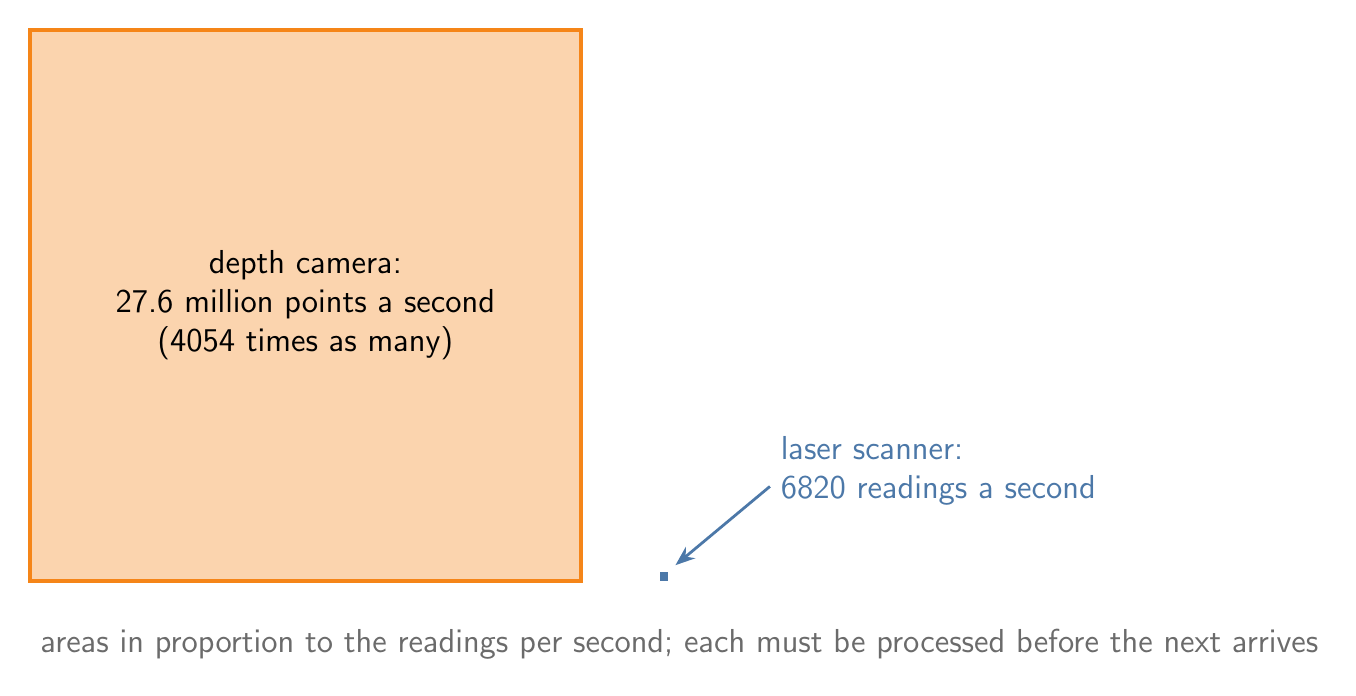
\begin{tikzpicture}
  \fill[corange!35] (0,0) rectangle (7.0,7.0); \draw[corange, line width=1.5pt] (0,0) rectangle (7.0,7.0);
  \fill[cblue] (8.0,0) rectangle (8.110,0.110);
  \draw[cblue, line width=1pt, -{Stealth[length=2.5mm]}] (9.4,1.2) -- (8.2,0.2);
  \node[note, font=\sffamily\large, text=cblue, anchor=west, align=left] at (9.4,1.4) {laser scanner:\\ 6820 readings a second};
  \node[note, font=\sffamily\large, text=black, align=center] at (3.5,3.5) {depth camera:\\ 27.6 million points a second\\ (4054 times as many)};
  \node[note, font=\sffamily\large, anchor=west, align=left] at (0,-0.8) {areas in proportion to the readings per second; each must be processed before the next arrives};
\end{tikzpicture}
\end{document}
